\section{ivmmod - WIP} \label{sec: ivmmod ex}
Adapted from Dr. Trudnowski example.
Shows how angle change `moves' entire system.
VTS option shows how variable time step method will adjust to capture dynamics.

\begin{figure}[H]
	\centering
	\footnotesize
	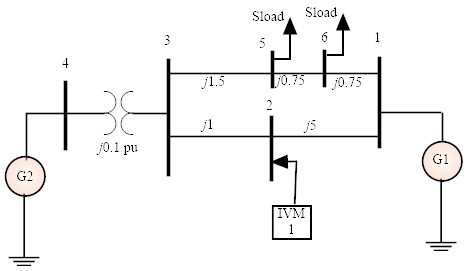
\includegraphics[width=.85\linewidth]{examples/ivmmod/ivmOneLine}
	\caption{System one-line diagram from run\_IVM.}
	\label{fig: ivm oneline}
\end{figure}%\vspace{-1 em}

\begin{figure}[H]
	\centering
	\footnotesize
	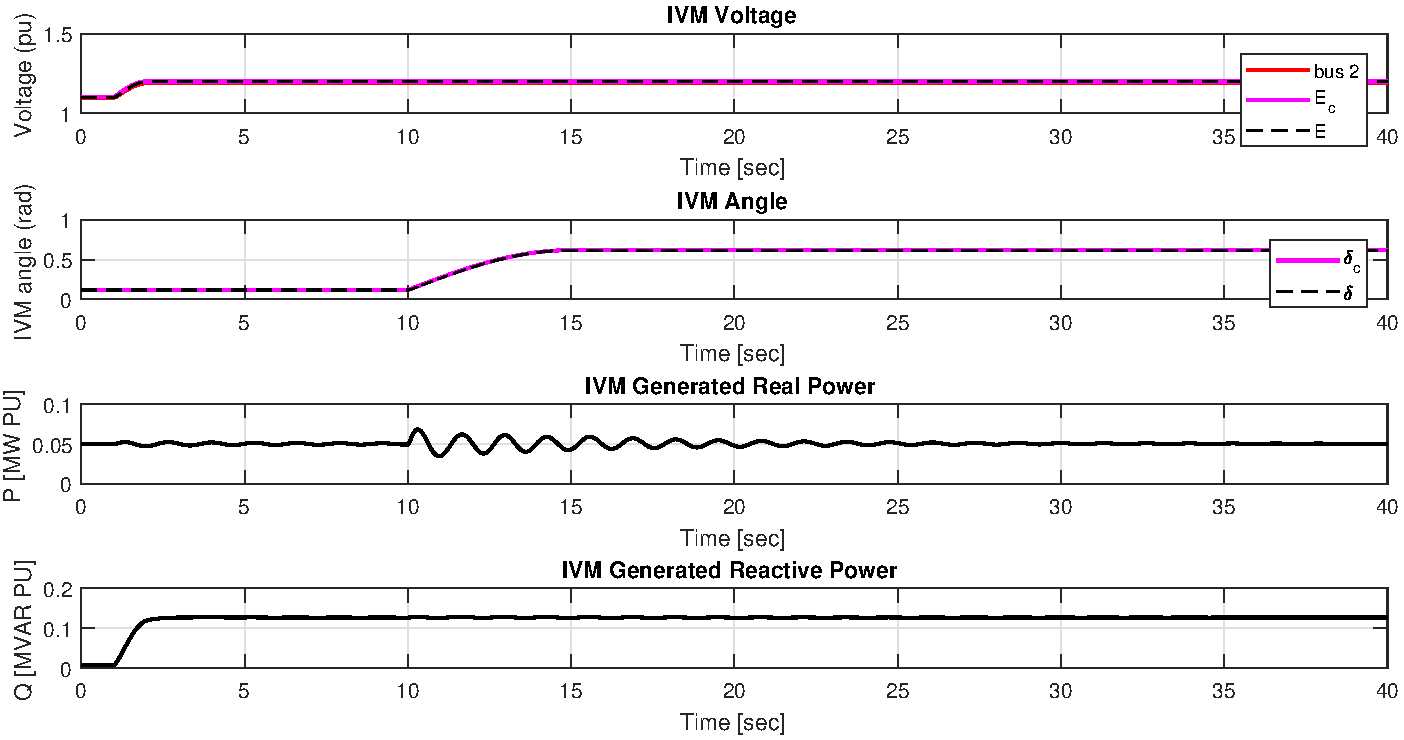
\includegraphics[width=\linewidth]{examples/ivmmod/ivm-vdelta}
	\caption{IVM action and resulting generator power output from run\_IVM.}
	\label{fig: ivm pw}
\end{figure}%\vspace{-1 em}
\pagebreak
All system angles change when the angle is perturbed at $t=10$.
The desired outcome would be for the controlled machine to generate more real power, however, this is not the case.
\begin{figure}[H]
	\centering
	\footnotesize
	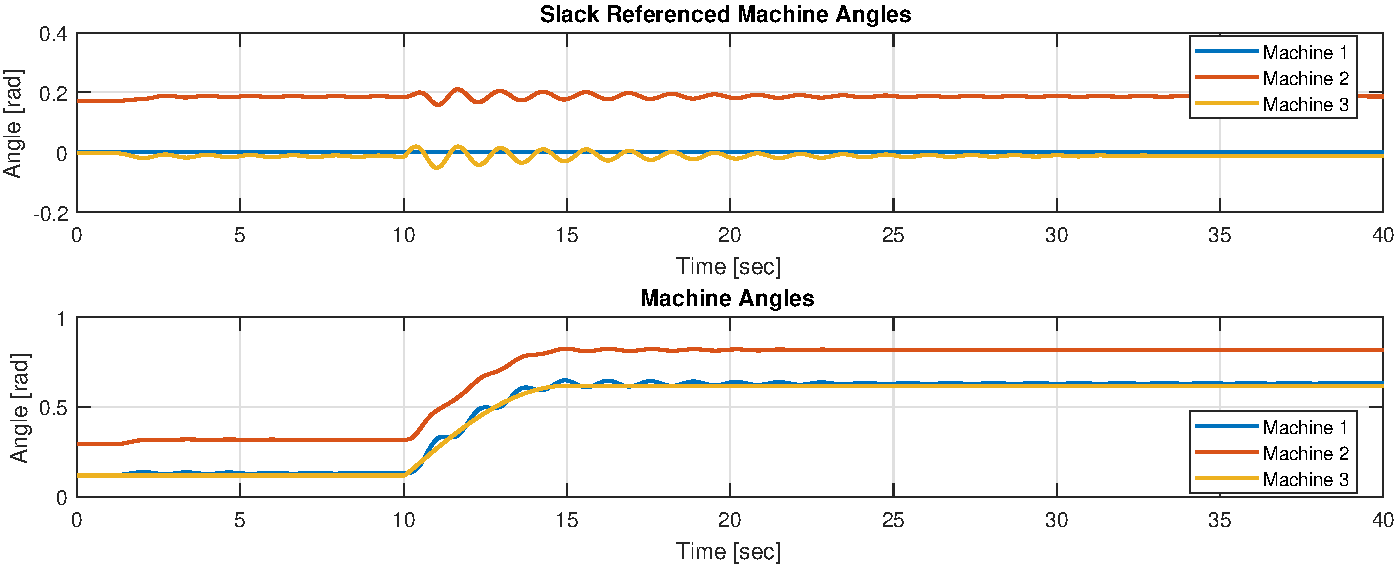
\includegraphics[width=\linewidth]{examples/ivmmod/ivm-angle}
	\caption{Machine angle comparisons from run\_IVM.}
	\label{fig: ivm angle}
\end{figure}%\vspace{-1 em}
